\chapter{Results and Discussion}

\section{Piezo1 as integrator of biomechanical events}
Piezo1 has been established as important mechanotransductive element \cite{Murthy2017} \cite{Gudipaty2017} in many different, multi-scale physiological  contexts, like blood pressure regulation [Zheng2018] and neuronal stem cell differentiation[Pathak2014]. Here we address the issue of transferability and try to determine, whether Piezo1 contributes significantly to mechanosensing in mesenchymal stem cells.\\



\begin{figure}
    \centering
    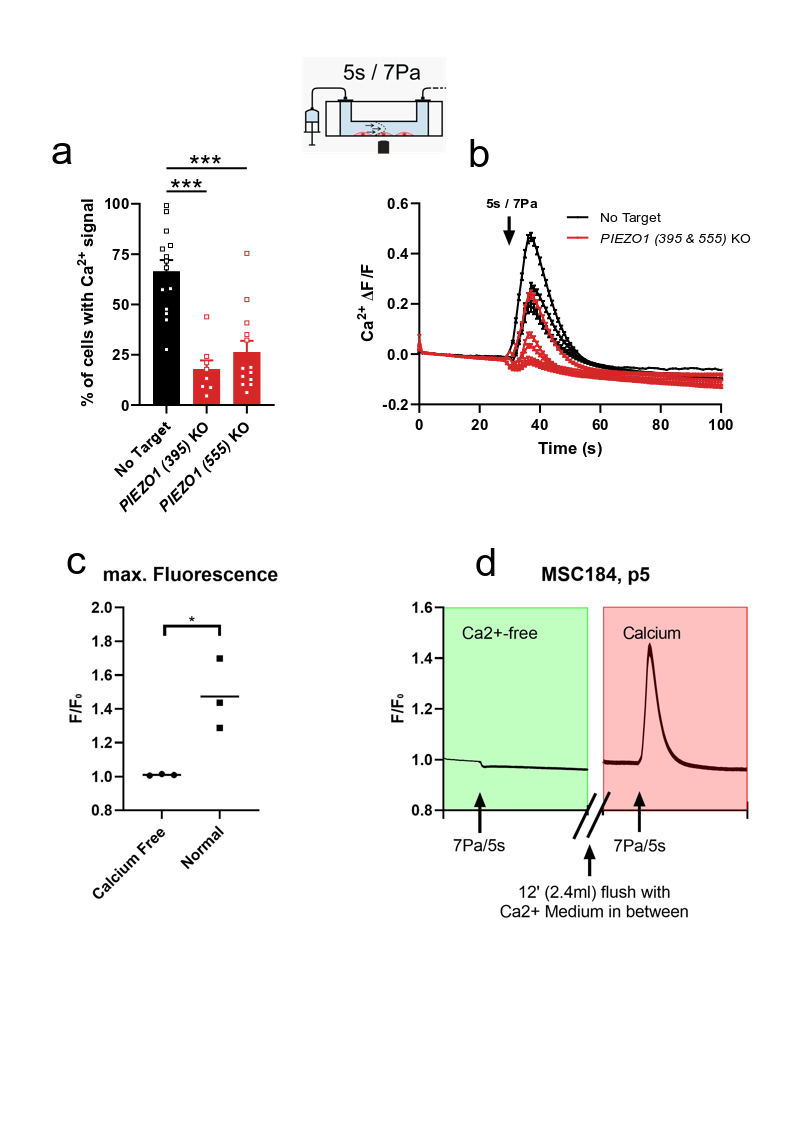
\includegraphics[width = 0.7\textwidth]{Combined_CalciumFree_KnockOut.png}
    \caption{Piezo1-mediated influx of extracellular Ca2+ confirmed as mechanotransductory event in MSC. \textit{Top:} Schematic drawing of Flowchamber. a.) Calcium-influx in response to fluidic shear pulse of 5s with an amplitude of 7Pa is significantly lower in two Piezo1-KO constructs, when compared to No Target-KO cell line. (Data points describe technical replicates, ***p$<$0.0001, ANOVA with Dunnette's multiple comparison test) b.) Same data as in previous graph with time-curve plotted shows that KO-constructs pooled exhibit lower peaks and less area under the curve when comparing to No Target-KO cell line. c.) Missing calcium-signal after application of shear stimulus, if no external calcium-ions are supplied. (n = 3, *p $<$ 0.05, Student's t-test) d.) Representative donor measurement of medium comparison shows complete lack of calcium-influx response after shear stimulus with calcium-free medium as opposed by calcium-containing response. (Data contains pooled data of 4 technical replicates and is mean $\pm$ SEM)}
    \label{fig:Calcium}
\end{figure}


\subsection{\Piezo{} contributes to mechanosensing in MSCs}

In this experiment we want to elucidate whether membrane-bound \Piezo{} contributes significantly to the mechanosensing in mesenchymal stem cells. Calcium influx is established as a almost instant trigger for the propagation of mechanotransduction.

The insight from before relies on the assumption of the calcium-ion-influx being a primary consequence of Piezo1 opening, as opposed by the hypothesis that activate Piezo1 channels might elicit a secondary reaction, like release of ionic calcium from intracellular storages. To test this assumption, we designed an experiment, with the flushding medium as the experimental condition.\\
Flushing the same flowchamber twice, one time with calcium-free ACSF and another time with normal ACSF, we saw an average of 40\% increase in measured $F_{max}/F_{0}$ levels in the second measurement, while a detectable impulse response during the measurement with calcium-free ACSF was missing .\par

To conclude, this result combined with the results from before shows that not only do MSC have mechanosensing capabilities, but the associated extracellular calcium ion influx is \Piezo{} mediated. 

Regarding validity of this experiment, one should always keep the following in mind: The strength of this method is also its weakness, as we can investigate here isolated mechanical effects here that are likely to be accompanied with confounding chemical stimuli in the physiological context.


Here in Balgrist we have access to a special methodology, named the flowchamberMaking use of in-house developed flowchambers, we measured an increase of maximal relative fluorescence levels directly relating to shear stress. This supports the notion of calcium influx as immediate reaction to shear in mesenchymal stem cells, similar to what we would expect in tendon. Follow up experiments with two Piezo1 knock-out cell lines (P1-395, P1-555) indicated that Piezo1 is the main trigger, as calcium-response was largely lacking when compared to negative control (No Target KO Cell line)

\section{Piezo1 and the extracellular matrix}

Preliminary mass spectroscopy secretome analysis of \Yoda-treated cells showed a distinct decrease in core extracellular matrix (ECM) components, such as alpha-1 type I collagen(\colone), Fibronectin-1 (\textsc{Fn1}) and finally alpha-1 type III collagen (\colthree) (Not shown here).
This inspired further investigation into this matter.\par

We stimulated Piezo1 during 30 minutes following the protocol described earlier \myworries{REF}.
By measures of SDS-PAGE, we were able to compare intracellular protein content of \Yoda-treated cells with control. There we saw a \myworries{very sharp} decline in \colone-content, which corroborate the findings from the secretome analysis. Surprisingly, the effects were not only marked by fast onset but also of long-lasting nature, since the effect of a singular 30 minutes \Yoda-exposition remained the same three days after intervention. \par

We also looked at mRNA representation of identical samples through qRT-PCR, where we biased our analysis towards \colone{ }, \colthree{}, \textsc{Fn}1 and Interleukin-6 to confirm our prior results.  All measurements were normalised against negative control samples harvested immediately after the intervention.\\
While we were not able to produce a significant result in any time point or gene, we saw a tendency of relative decrease in \colone{} over three days when comparing Piezo1-activation group with negative control group. It is likely to produce a significant result in day 3 with increasing sample size. Quite remarkably, the rapid downregulation of Protein in day 1 is not mirrored in RNA concentration. This result is both unexpected and intriguing. The divergence between results from Western Blot and qRT-PCR introduces a new dimension, inspiring further research into the topic.

While the results were surprising, follow-up studies are required before we can make any sound conclusions. We have good reasons as to think why increased secretion or reduced gene expression would likely not be a valid explanation for the data at hand. RNA analysis does not show a decrease in gene transcription, which would be seen in a different gene expression profile. Mass spectroscopy analysis of conditioned medium of MSC does also show a decrease in the ECM proteins, thus making the explanation of increased secretion invalid. However, there are at least one different hypothesis that could lead to this result. The explanation includes a Piezo1-mediated protein degradation mechanism. For example, a cytosolic protease that relies on an ionic cofactor (e.g. Calcium) for effector-function would be straightforward explanation. 


\begin{figure}[ht]
    \centering
    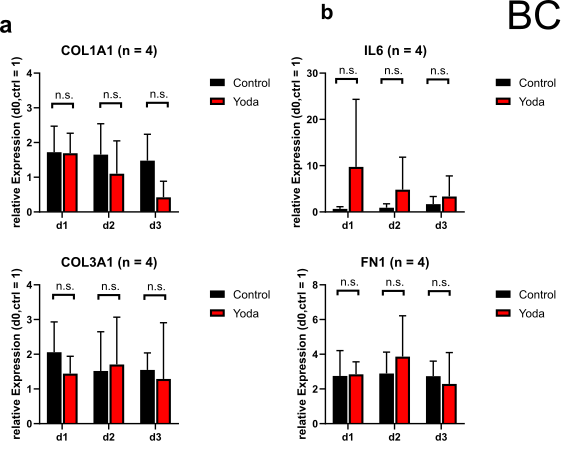
\includegraphics[scale = 0.6]{Collection.png}
    \caption{
    Modest adaptation on transcriptional level as consequence of Piezo1-Activation. \hfill \newline
    \textbf{a}: \colone{}
    \textbf{b}: IL-6
    \textbf{c}: \colthree{}
    \textbf{d}: \textsc{Fn}1. 
    (All Experiments: n = 4). 
    }
    \label{fig:my_label}
\end{figure}


\begin{figure}[htbp]
  \centering
  \includesvg[width=\linewidth]{200205_WesternBlotQuantified_YodaExp_Col1a1.svg}
  \caption{svg image}
\end{figure}


\section{\Piezo and osteogenic differentiation}

\begin{figure}[htbp]
  \centering
  \includesvg[width = 0.7\linewidth]{Osteogenic_PCR_Yoda.svg}
  \caption{svg image}
\end{figure}

Something that is reported in literature Here I'm basically going to mention that due to long-term nature of the effect we suspected differentiation. Since Proteins investigated are heavily implicated with Osteogenic differentiation, we looked into osteogenic differentiation. Enter Graph. Even though some tendency can be seen, results of those markers are not significant. 

\section{Reversibility of Piezo1-stimulation}


\begin{figure}
    \centering
    \includesvg{Collective_Long_v1.svg}
    \caption{Tendency of Yoda-effect still visible 7 days after intervention. After 3 days, medium was changed and either supplemented with 10\% FBS (denoted with S+) or serum-free (denoted with S-). (n = 1)}
    \label{fig:my_label}
\end{figure}

In this experiment we wanted to investigate whether the effects seen before would recover after some time and the cells enter a state of pre-intervention homeostasis. One technical issue that we had to solve in this experiment, was the fact that a significant amount of cells showed signs of distress and apoptosis after Yoda1-intervention. In order to allow for sufficient cell survival until we would harvest the cell for analysis, we adapted the protocol from the previous experiment, such that we changed the medium after three days. Half of the cells received serum free MEM\textalpha{}, whereas the other half was administered MEM\textalpha{} with 10\% FBS. 
While we can clearly see that cells proliferate again in reaction to FBS, they don't seem to recover anymore from Piezo1-activation. \myworries{Wrong Text here}

\section{Excursion: Biostability of Yoda1 and Piezo1 mediated apoptosis}
\label{sec:biostability}
We realised that 3 days after the intervention, there was a large decrease in cell count in Yoda1-treated cells when compared to negative control. Next to Piezo1 being implicated in this pro-apoptotic effect, an intrinsic cytotoxicity of Yoda1 could also be an explanation. To test this hypothesis, Uli, in an explorative experiment, exposed both Piezo1-KO and NoT Cell Lines to Yoda1, which showed that the apoptotic effect is dependent on Piezo1 Expression. (Not shown)

\begin{figure}
    \centering
    \includesvg[width = \linewidth]{Yoda_Apoptosis.svg}
    \caption{Light microscopy picture of cells 7 days after intervention both cultured serum-free. Observe the round, \myworries{apoptotic} morphology in the Yoda1-treated samples.}
    \label{fig:yoda_apop}
\end{figure}